\section{The Recall Cliff}
\label{sec:cliff}

\subsection{Detector Operating Points}
Table~\ref{tab:detector} and Fig.~\ref{fig:detector} report the two detectors on
ResNet-18/BadNets models at poison rates of 1\%, 5\%, and 10\%. Three features of
these measurements motivate the rest of the paper.

First, recall is not free. Spectral signatures flags a fixed budget of $1.5N_p$
samples and recovers only 33.8\% of the poison at a 1\% poison rate, because the
top-scoring clean samples crowd out poison at that scale. Activation clustering
recovers all of it at 1\% and 5\%, but at 10\% it returns an empty flag set: the
class-0 cluster no longer passes its size and silhouette tests, so the detector
reports that nothing is wrong at exactly the poison rate where the attack is
strongest.

Second, precision degrades as recall improves. At 5\%, activation clustering
flags 4{,}140 samples for 2{,}500 true poison (precision 0.60) and spectral
signatures flags 3{,}750 (precision 0.64). A removal method therefore receives a
forget set in which roughly one third of the entries are clean images.

Third, architecture matters. The same detectors on VGG-16-BN and MobileNetV2
produced degenerate outputs (no flags, or flags with no true positives) and are
excluded. Detector behaviour is not a property of the attack alone; it is a
property of the representation, which is why a controlled parameterisation of
detector output is more portable than a fixed threshold.

\begin{table}[t]
\centering
\caption{Measured detector operating points: the noisy forget sets that motivate the grid.}
\label{tab:detector}
\footnotesize
\begin{tabular}{cccccc}
\toprule
\textbf{Poison} & \textbf{Det.} & \textbf{Flagged} & \textbf{TP} & \textbf{Precision} & \textbf{Recall} \\
\midrule
1\% & AC & 507 & 500 & 0.986 & 1.000 \\
1\% & SS & 750 & 169 & 0.225 & 0.338 \\
5\% & AC & 4,140 & 2,500 & 0.604 & 1.000 \\
5\% & SS & 3,750 & 2,411 & 0.643 & 0.965 \\
10\% & AC & 0 & 0 & -- & -- \\
10\% & SS & 7,500 & 2,400 & 0.320 & 0.480 \\
\bottomrule
\end{tabular}
\par\vspace{1pt}\footnotesize\raggedright Detector output on a ResNet-18/BadNets model; TP is the number of true poison samples among the flags. At 10\% poison, AC returns an empty flag set (no cluster passes its size/silhouette test), i.e.\ $r=0$: the detector, not the removal method, is the binding constraint. VGG-16-BN and MobileNetV2 detector runs were degenerate (no flags or no true positives) and are excluded.
\end{table}


\begin{figure}[t]
\centering
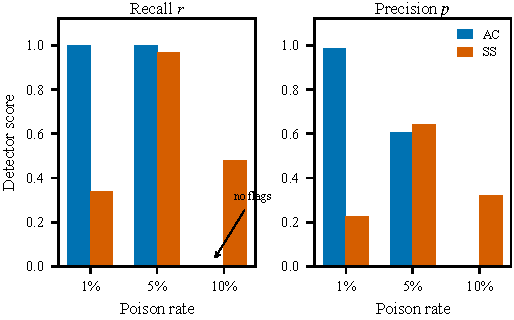
\includegraphics[width=\columnwidth]{fig10_detector.pdf}
\caption{Detector recall and precision on ResNet-18/BadNets at three poison
rates. Activation clustering (AC) returns no flags at 10\% poison; spectral
signatures (SS) is limited by its fixed $1.5N_p$ flag budget at 1\%.}
\label{fig:detector}
\end{figure}

\subsection{Deletion Collapses Between $r{=}0.95$ and $r{=}0.90$}
Fig.~\ref{fig:cliff} and Table~\ref{tab:e1grid} give the central result.
Retraining on the retained set is essentially perfect when the forget set
contains every poisoned sample: ASR $1.68\pm0.26\%$ at $r{=}1$, with clean
accuracy $88.67\%$ against a gold value of $88.59$--$88.77\%$. It remains low at
$r{=}0.95$ (ASR $2.84\pm0.73\%$), but the clean accuracy of that model is
$84.58\%$, four points below gold, so the joint criterion already fails. At
$r{=}0.90$ the backdoor is fully back: ASR $100.00\pm0.00\%$ with clean
accuracy $88.80\%$. From there down to $r{=}0.25$ the ASR stays between 99.63
and 100.00\%. The transition is not gradual. Removing 2{,}375 of 2{,}500 poison
samples leaves a model that still cannot be attacked at a useful rate; removing
2{,}250 does not.

The $r{=}0.95$ cell deserves a comment because it looks like a counterexample.
No clean samples are removed there ($p{=}1$), so the four-point clean-accuracy
drop cannot be a false-positive effect. It is a property of retraining on a set
that still contains 125 poison samples, and we did not isolate the mechanism. We
report it as measured; the practical consequence is the same, because the joint
criterion is what a deployment decision would use. It is also the reason
$\rstar{=}1.00$ rather than $0.95$: the ASR cliff is at 0.90, but the success
cliff is at 1.00.

\begin{figure}[t]
\centering
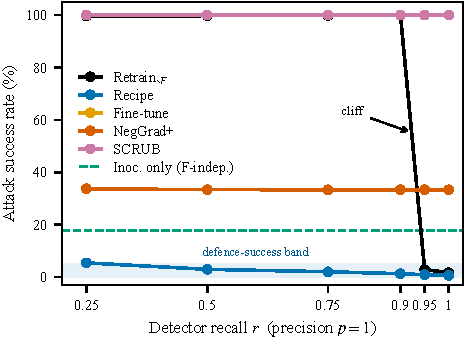
\includegraphics[width=\columnwidth]{fig2_e1_cliff.pdf}
\caption{Attack success after removal as a function of detector recall at
precision 1.0 (mean over three seeds). Deletion is flat at 100\% for
$r\leq0.90$ and drops only when every poisoned sample is removed. The dashed
line is the inoculation-only baseline, which uses no forget set; the shaded band
is the 5\% success threshold.}
\label{fig:cliff}
\end{figure}

\begin{table*}[t]
\centering
\caption{E1: the recall--precision grid. Deletion meets the success criterion only at full recall; repair$+$inoculation holds ASR below 5\% down to $r{=}0.5$.}
\label{tab:e1grid}
\scriptsize
\begin{tabular}{ccrccccc}
\toprule
\textbf{$r$} & \textbf{$p$} & \textbf{$|\mathcal{F}|$} & \textbf{Retrain$_{\setminus F}$} & \textbf{Fine-tune} & \textbf{NegGrad+} & \textbf{SCRUB} & \textbf{Recipe} \\
\midrule
1.00 & 1.0 & 2,500 & \textbf{1.68$\pm$0.26} & 100.00$\pm$0.00 & 33.33$\pm$57.74 & 100.00$\pm$0.00 & \textbf{0.63$\pm$0.21} \\
0.95 & 1.0 & 2,375 & \textbf{2.84$\pm$0.73} & 100.00$\pm$0.00 & 33.33$\pm$57.74 & 100.00$\pm$0.00 & \textbf{0.90$\pm$0.11} \\
0.90 & 1.0 & 2,250 & 100.00$\pm$0.00 & 100.00$\pm$0.00 & 33.33$\pm$57.74 & 100.00$\pm$0.00 & \textbf{1.27$\pm$0.58} \\
0.75 & 1.0 & 1,875 & 99.78$\pm$0.22 & 100.00$\pm$0.01 & 33.33$\pm$57.74 & 100.00$\pm$0.00 & \textbf{2.03$\pm$1.32} \\
0.50 & 1.0 & 1,250 & 99.76$\pm$0.31 & 100.00$\pm$0.01 & 33.35$\pm$57.72 & 100.00$\pm$0.00 & \textbf{2.95$\pm$0.78} \\
0.25 & 1.0 & 625 & 99.63$\pm$0.58 & 99.97$\pm$0.02 & 33.71$\pm$57.41 & 100.00$\pm$0.00 & 5.42$\pm$1.82 \\
0.90 & 0.9 & 2,500 & 99.99$\pm$0.01 & 100.00$\pm$0.00 & 33.33$\pm$57.74 & 100.00$\pm$0.00 & \textbf{1.16$\pm$0.43} \\
0.90 & 0.7 & 3,214 & 99.99$\pm$0.02 & 100.00$\pm$0.00 & 33.33$\pm$57.74 & 100.00$\pm$0.00 & \textbf{1.90$\pm$0.34} \\
0.50 & 0.9 & 1,389 & 99.77$\pm$0.21 & 99.97$\pm$0.03 & 33.35$\pm$57.72 & 100.00$\pm$0.00 & \textbf{3.57$\pm$0.40} \\
0.50 & 0.7 & 1,786 & 99.90$\pm$0.15 & 99.99$\pm$0.01 & 33.34$\pm$57.73 & 100.00$\pm$0.00 & \textbf{2.59$\pm$1.03} \\
\bottomrule
\end{tabular}
\par\vspace{1pt}\scriptsize\raggedright ASR (\%) after removal, mean$\pm$s.d.\ over three seeds; \textbf{bold} marks mean ASR $\leq5\%$ (the ASR half of defence success; clean accuracy is checked in Table~\ref{tab:success}). $|\mathcal{F}|$ is reported for the seed-0 draw (identical across seeds up to rounding). NegGrad+ is bimodal across seeds: two seeds drive ASR to $\approx  0$ while collapsing clean accuracy to 75--86\% at $p{=}1$ (in the four $p<1$ cells one of those seeds collapses further to 10\%), one stays fully inert (ASR 100\%); the mean and s.d.\ describe the mixture, not a stable operating point.
\end{table*}


\subsection{The Cliff Is a Function of Residual Poison}
A separate block (E2) varies the fraction of poison left in the training set
directly, without a detector and without simulated false positives.
Table~\ref{tab:residual} and Fig.~\ref{fig:residual} show the result for the four
architecture--attack combinations. With 0\%, 25\%, 50\%, or 75\% of the poison
still present, ASR is between 99.83\% and 100.00\% in every cell. At complete
removal it falls to 0.59--1.22\%. Clean accuracy varies by at most 0.9 points
across the five fractions within each setting, so the collapse is not a
side-effect of a damaged network. The shape is a step, and the step is located at
zero residual poison. This is the same phenomenon as the grid's $r{=}1$
boundary, seen from the other side: what matters is not how much poison was
deleted but whether any remains. The absolute clean accuracies in E2 are
89.2--90.5\%, slightly above the E1 gold values, because the block was trained
separately; the ASR pattern, not the absolute accuracy, is the object of
comparison.

\begin{table}[t]
\centering
\caption{E2: the cliff is a step function of residual poison, not of the amount deleted.}
\label{tab:residual}
\footnotesize
\setlength{\tabcolsep}{4.5pt}
\begin{tabular}{lcccccc}
\toprule
\textbf{Setting} & \textbf{0\%} & \textbf{25\%} & \textbf{50\%} & \textbf{75\%} & \textbf{100\%} & \textbf{Gold} \\
\midrule
R18/BadNets & 99.83 & 99.98 & 99.94 & 100.00 & 1.21 & 90.3 \\
R18/Blend & 99.99 & 99.97 & 99.97 & 99.86 & 0.64 & 90.2 \\
VGG/BadNets & 100.00 & 99.99 & 100.00 & 100.00 & 1.22 & 89.7 \\
VGG/Blend & 99.97 & 100.00 & 99.94 & 99.98 & 0.59 & 89.7 \\
\bottomrule
\end{tabular}
\par\vspace{1pt}\footnotesize\raggedright ASR (\%) versus the fraction of poison left in the training set after deletion. The last column is the gold retrain's clean accuracy for that setting; across the five residual fractions, clean accuracy varies by at most 0.9 points in every setting, so the cliff is not an accuracy artefact.
\end{table}


\begin{figure}[t]
\centering
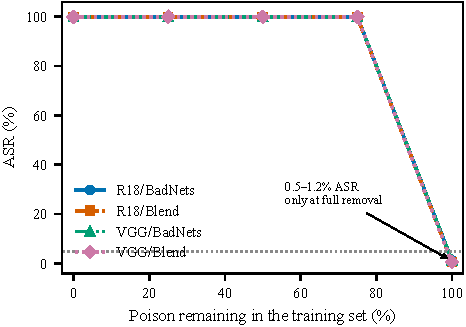
\includegraphics[width=\columnwidth]{fig4_e2_residual.pdf}
\caption{ASR versus the fraction of poison remaining in the training set, for
four architecture--attack combinations. The curve is flat until the poison is
completely gone.}
\label{fig:residual}
\end{figure}

\subsection{Precision Is Secondary to Recall}
The precision axis is much flatter than the recall axis. At fixed $r{=}0.90$,
moving from $p{=}1.0$ to $p{=}0.9$ or $p{=}0.7$ enlarges the forget set from
2{,}250 to 2{,}500 or 3{,}214 samples, and deletion's ASR moves from
$100.00\%$ to $99.99\%$ in both cases. At fixed $r{=}0.50$, $p{=}0.7$ gives
$99.90\%$ against $99.76\%$ at $p{=}1.0$. For the recipe the same manipulation is
visible but small: ASR goes from $1.27\%$ to $1.90\%$ at $r{=}0.9$ and from
$2.95\%$ to $2.59\%$ at $r{=}0.5$, with no consistent direction. Deleting extra
clean data costs some accuracy (the recipe's clean accuracy moves within about
0.6 points), but it neither rescues nor destroys a removal that is otherwise
working.

The asymmetry has a simple reading. A false positive is a clean sample removed
from training, which the network can absorb if the dataset is large. A false
negative is a poisoned sample kept in training, which re-installs the association
the removal was meant to break. At a 5\% poison rate, the largest precision
penalty we test ($p{=}0.7$) adds 714 clean samples to a 50{,}000-sample training
set, a 1.4\% perturbation. The smallest recall penalty we test ($r{=}0.95$)
leaves 125 poison samples, which is enough to matter. Detector engineering for
removal should therefore optimise recall first and treat precision as a budget
constraint.

\subsection{The Other Method Families}
The remaining families do not merely fail at low recall; most of them fail at
full recall as well.

\method{Fine-tune} never removes the backdoor: ASR is $100.00\pm0.00\%$ at
$r{=}1$ and above 99.96\% in every other cell, while clean accuracy is
unaffected ($89.02\%$). Three epochs on the retained set reinforce whatever the
poisoned model already represents.

\method{NegGrad+} is bimodal. In most cells the mean ASR is $33.33\%$ with a
standard deviation of $57.74$, which is the signature of two seeds near zero and
one seed at 100\%. Where it does suppress the backdoor, it does so by damaging the
model: clean accuracy is $79.90\pm7.55\%$ at $r{=}1$, and at $(r,p)=(0.9,0.9)$ it
is $54.23\pm38.31\%$. Under the joint criterion it never succeeds, and the
bimodality means that a single-seed evaluation of this method would be
uninformative in either direction.

\method{SCRUB} leaves ASR at $100.00\pm0.00\%$ in every one of the ten cells.
Its clean accuracy is also unstable, from $65.76\pm20.17\%$ at $r{=}1$ to
$86.07\pm2.59\%$ at $r{=}0.25$. The teacher-student objective assumes that the
forget set is the poison; when it is not, the student is trained to match the
teacher on poison and the backdoor survives.

\emph{Inoculation only} is the interesting baseline. It uses no forget set at
all, so it cannot degrade with recall, and it does reduce ASR from near 100\% to
$17.67\%$ with clean accuracy $88.41\%$. That is a real effect, but it is above
the 5\% threshold and therefore not a success by our criterion. It also shows
that inoculation alone is not sufficient on CIFAR-10; the combination with label
repair is what produces the recipe's numbers.

The recipe holds ASR between $0.63$ and $2.95\%$ for every cell with
$r\geq0.5$ and at $p{=}1$, and between $1.16$ and $3.57\%$ for the $p<1$ cells,
with clean accuracy between 87.37 and 88.00\%. It degrades at $r{=}0.25$
($5.42\pm1.82\%$) and is the only method whose failure, when it comes, is a
gradual loss of margin rather than a return of the backdoor. The reason is
structural: its inoculation stage does not require the forget set to be
complete. We return to the cost of that property in Section~\ref{sec:general}.

\subsection{Success Counts and the Tolerance $\rstar$}
Table~\ref{tab:success} and Fig.~\ref{fig:success} convert the grid into the
joint criterion. Deletion succeeds on all three seeds in exactly one cell,
$(r,p)=(1,1)$, and on no seed anywhere else; its tolerance is
$\rstar{=}1.00$. Fine-tuning, NegGrad+, and SCRUB have no successful cell.
The recipe succeeds on 3/3 seeds in eight of the ten cells and on 2/3 in the two
$r{=}0.5$ and $r{=}0.25$ cells at $p{=}1$. At $r{=}0.5$ one seed misses the
clean budget by $0.09$ points. At $r{=}0.25$ one seed exceeds the ASR threshold
($7.49\%$), and the three-seed mean does too ($5.42\%$), so that cell is outside
the mean rule as well. At $(0.5,1.0)$ the mean clean accuracy is
$87.37\%$ against a gold mean of $88.67\%$, which is inside the two-point budget,
so the mean definition of Eq.~\eqref{eq:rstar} gives $\rstar{=}0.50$. An
all-seeds rule would instead give $0.75$, and Table~\ref{tab:success} reports the
counts so that both readings are visible.

\begin{table*}[t]
\centering
\caption{Defence-success counts and the recall tolerance $r^{*}$.}
\label{tab:success}
\scriptsize
\begin{tabular}{lccccccccccc}
\toprule
\textbf{Method} & \multicolumn{10}{c}{\textbf{Successes (of 3) per $(r,p)$ cell, ordered as in Table~\ref{tab:e1grid}}} & \textbf{$\rstar$} \\
\midrule
Retrain$_{\setminus F}$ & 3 & 0 & 0 & 0 & 0 & 0 & 0 & 0 & 0 & 0 & 1.00 \\
Fine-tune & 0 & 0 & 0 & 0 & 0 & 0 & 0 & 0 & 0 & 0 & -- \\
NegGrad+ & 0 & 0 & 0 & 0 & 0 & 0 & 0 & 0 & 0 & 0 & -- \\
SCRUB & 0 & 0 & 0 & 0 & 0 & 0 & 0 & 0 & 0 & 0 & -- \\
Recipe & 3 & 3 & 3 & 3 & 2 & 2 & 3 & 3 & 3 & 3 & 0.50 \\
\bottomrule
\end{tabular}
\par\vspace{1pt}\scriptsize\raggedright Number of seeds (of 3) meeting both criteria (ASR $\leq5\%$ and clean accuracy within 2 points of the gold retrain), in the order of Table~\ref{tab:e1grid}. $\rstar$ is the smallest $p{=}1$ recall at which the three-seed mean meets both criteria (Eq.~\eqref{eq:rstar}); the counts allow the stricter all-seeds rule to be read off, and under it the recipe's tolerance would be $0.75$. At $(0.5,1.0)$ the recipe's mean clean accuracy is $87.37\%$ against a gold mean of $88.67\%$, inside the budget, although one seed misses it by $0.09$ points. Gold clean accuracy: 88.59 / 88.65 / 88.77.
\end{table*}


\begin{figure}[t]
\centering
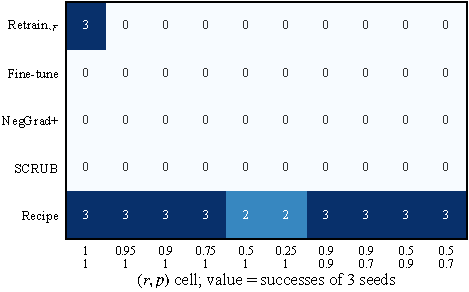
\includegraphics[width=\columnwidth]{fig3_success_map.pdf}
\caption{Number of seeds (of three) meeting both success criteria in each
$(r,p)$ cell. Deletion is dark everywhere except the full-recall corner; the
recipe is dark everywhere except the two lowest-recall cells at $p{=}1$.}
\label{fig:success}
\end{figure}

\subsection{The Grid in Four Views}
Fig.~\ref{fig:views} rearranges the ten cells along four axes. Panel (a) follows
clean accuracy across recall at precision 1.0. Deletion sits on the gold line at
every recall except $r{=}0.95$, where it loses 4.09 points, and $r{=}1$, where it
\emph{is} the gold; SCRUB's damage is concentrated at full recall, where its
three seeds are 57.05\%, 88.83\%, and 51.41\% (mean 65.76\%); the recipe stays
within 1.3 points across the whole range. Panels (b) and (c) are the precision
axes at $r{=}0.9$ and $r{=}0.5$; both are almost flat. Moving $p$ from 1.0 to 0.7
changes deletion's ASR by at most 0.3 points and the recipe's by at most 0.7,
while fine-tuning and SCRUB remain at 100\% and NegGrad+ near its bimodal mean of
33.3\%. Panel (d) isolates the one exception: at $r{=}0.5$, NegGrad+'s clean
accuracy falls from 83.82\% at $p{=}1$ to 57.78\% at $p{=}0.7$. A larger forget
set gives its ascent step more clean samples to damage. That is the only visible
precision effect in the grid, and it belongs to a method that fails at every
precision.

\begin{figure*}[t]
\centering
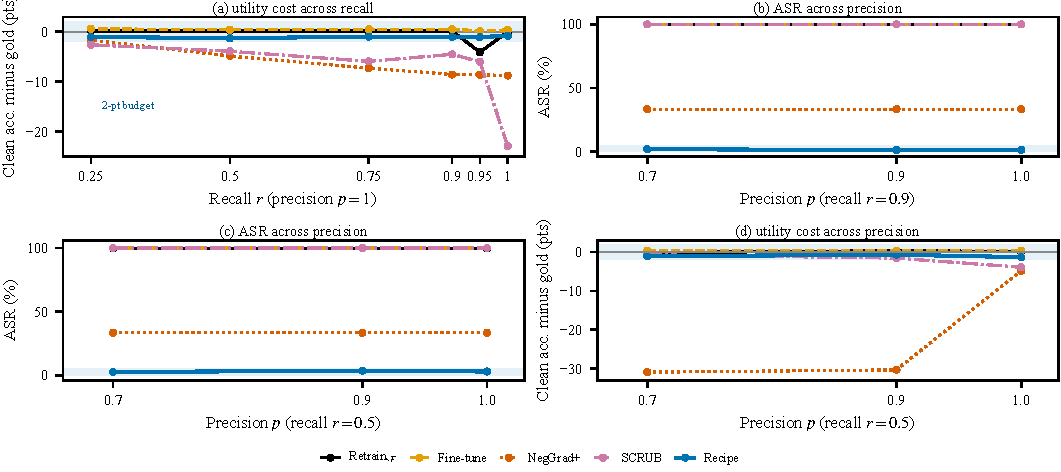
\includegraphics[width=\textwidth]{fig16_grid_views.pdf}
\caption{The E1 grid rearranged. (a) Clean accuracy relative to gold across
recall at $p{=}1$; the shaded band is the two-point budget. (b), (c) ASR across
precision at $r{=}0.9$ and $r{=}0.5$. (d) Clean accuracy relative to gold across
precision at $r{=}0.5$. The recall axis moves every method; the precision axes
move only NegGrad+.}
\label{fig:views}
\end{figure*}

\subsection{Real Detector Columns}
The grid uses simulated forget sets. Table~\ref{tab:e6} checks the conclusion
against the detectors' raw flag sets, with no simulation. Activation clustering
flags exactly the poison at 5\% in this run, and the resulting deletion is a
success (ASR $1.62\%$, clean $88.70\%$). Spectral signatures recovers 83.4\% of
the poison at precision 0.834, and the same deletion method fails completely:
ASR $99.87\%$ with clean accuracy $88.89\%$. The SS column uses the detector's
raw flag set (2{,}500 flags) rather than the fixed $1.5N_p$ budget of
Table~\ref{tab:detector}, so its operating point differs from that table. The
recipe succeeds in both columns
($0.70\%$ and $1.43\%$), and SCRUB fails in both ($100.00\%$). This is the
cleanest statement of the paper's practical claim: a 16.6\% recall shortfall,
which would be an unremarkable detector result, is enough to make the strongest
deletion method useless.

\begin{table}[t]
\centering
\caption{E6: realistic detector columns reproduce the simulated grid.}
\label{tab:e6}
\footnotesize
\begin{tabular}{lcccc}
\toprule
\textbf{Method} & \textbf{Recall} & \textbf{Precision} & \textbf{Clean} & \textbf{ASR} \\
\midrule
Retrain$_{\setminus F}$ & 1.000 & 1.000 & 88.70 & 1.62 \\
SCRUB & 1.000 & 1.000 & 61.37 & 100.00 \\
Recipe & 1.000 & 1.000 & 88.04 & 0.70 \\
Retrain$_{\setminus F}$ & 0.834 & 0.834 & 88.89 & 99.87 \\
SCRUB & 0.834 & 0.834 & 86.89 & 100.00 \\
Recipe & 0.834 & 0.834 & 88.18 & 1.43 \\
\bottomrule
\end{tabular}
\par\vspace{1pt}\footnotesize\raggedright Removal driven by the detectors' \emph{raw} flag sets (no simulation), seed 0. AC flags exactly the poison here; SS trades 16.6\% of recall for 16.6\% precision. Deletion inherits the detector's recall error directly; repair$+$inoculation does not.
\end{table}

